\documentclass[12pt,a4paper]{report}

% -----------------------------------------------
%  PACKAGES
% -----------------------------------------------
\usepackage[utf8]{inputenc}
\usepackage[T1]{fontenc}
\usepackage{lmodern}
\usepackage{microtype}
\usepackage{graphicx}
\usepackage{float}
\usepackage{subcaption}
\usepackage{hyperref}
\usepackage{geometry}
\usepackage{titlesec}
\usepackage{setspace}
\usepackage{fancyhdr}
\usepackage{amsmath}
\usepackage{amssymb}
\usepackage{booktabs}
\usepackage{array}
\usepackage{xcolor}
\usepackage{listings}
\usepackage{caption}
\usepackage{enumitem}
\usepackage{mdframed}
\usepackage{tcolorbox}
\usepackage{tikz}
\usetikzlibrary{shapes.geometric, arrows.meta, positioning, calc}
\usepackage{pgfplots}
\pgfplotsset{compat=1.18}
\usepackage{multirow}
\usepackage{longtable}
\usepackage{pdflscape}
\usepackage{afterpage}
\usepackage{abstract}

% -----------------------------------------------
%  PAGE GEOMETRY
% -----------------------------------------------
\geometry{
    a4paper,
    top=25mm,
    bottom=25mm,
    left=30mm,
    right=25mm
}

% -----------------------------------------------
%  HEADER / FOOTER
% -----------------------------------------------
\pagestyle{fancy}
\fancyhf{}
\fancyhead[L]{\small Enabling Deep Supervision in FFLUNet}
\fancyhead[R]{\small IIT Kharagpur -- Internship Report}
\fancyfoot[C]{\thepage}
\renewcommand{\headrulewidth}{0.4pt}

% -----------------------------------------------
%  CHAPTER / SECTION FORMATTING
% -----------------------------------------------
\titleformat{\chapter}[display]
  {\normalfont\bfseries\LARGE}
  {\chaptertitlename\ \thechapter}{14pt}{\LARGE}
\titlespacing*{\chapter}{0pt}{0pt}{20pt}

\titleformat{\section}
  {\normalfont\bfseries\large}{\thesection}{1em}{}
\titleformat{\subsection}
  {\normalfont\bfseries\normalsize}{\thesubsection}{1em}{}

% -----------------------------------------------
%  CODE LISTING STYLE
% -----------------------------------------------
\definecolor{codebg}{RGB}{248,248,248}
\definecolor{codeframe}{RGB}{200,200,200}
\definecolor{codecomment}{RGB}{100,100,100}
\definecolor{codekeyword}{RGB}{0,0,180}
\definecolor{codestring}{RGB}{163,21,21}

\lstdefinestyle{pythonstyle}{
  backgroundcolor=\color{codebg},
  commentstyle=\color{codecomment}\itshape,
  keywordstyle=\color{codekeyword}\bfseries,
  stringstyle=\color{codestring},
  basicstyle=\ttfamily\footnotesize,
  breakatwhitespace=false,
  breaklines=true,
  captionpos=b,
  keepspaces=true,
  numbers=left,
  numbersep=6pt,
  numberstyle=\tiny\color{gray},
  showspaces=false,
  showstringspaces=false,
  showtabs=false,
  tabsize=4,
  frame=single,
  rulecolor=\color{codeframe},
  language=Python
}
\lstset{style=pythonstyle}

% -----------------------------------------------
%  HYPERLINK SETUP
% -----------------------------------------------
\hypersetup{
    colorlinks=true,
    linkcolor=blue!70!black,
    urlcolor=blue!70!black,
    citecolor=green!50!black,
    pdftitle={Enabling Deep Supervision in FFLUNet -- Internship Report},
    pdfauthor={[Your Name]},
}

% -----------------------------------------------
%  SPACING
% -----------------------------------------------
\onehalfspacing

% -----------------------------------------------
%  TIKZ ARROW STYLE
% -----------------------------------------------
\tikzset{
  block/.style = {rectangle, draw, fill=blue!10,
    text width=5.5cm, text centered, rounded corners, minimum height=1cm},
  smallblock/.style = {rectangle, draw, fill=green!10,
    text width=3.5cm, text centered, rounded corners, minimum height=0.8cm},
  dsblock/.style = {rectangle, draw, fill=orange!15, dashed,
    text width=3.5cm, text centered, rounded corners, minimum height=0.8cm},
  arrow/.style = {thick,->,>=stealth},
  line/.style  = {thick,-,>=stealth},
}

% -----------------------------------------------
%  BEGIN DOCUMENT
% -----------------------------------------------
\begin{document}

% ==================================================
%  TITLE PAGE
% ==================================================
\begin{titlepage}
\begin{center}
    \vspace*{0.5cm}

    % If you have the IIT KGP logo, replace the placeholder below:
    % \includegraphics[width=0.22\textwidth]{iitkharagpur_logo.png}\\[0.5cm]
    \rule{\linewidth}{0.5mm}\\[0.3cm]

    {\LARGE \bfseries Indian Institute of Technology Kharagpur}\\[0.2cm]
    {\large Department of Computer Science and Engineering}\\[0.1cm]
    \rule{\linewidth}{0.5mm}\\[1.2cm]

    {\Huge \bfseries Enabling Deep Supervision\\[0.3cm] in FFLUNet}\\[0.8cm]

    {\Large \textit{Summer Research Internship Report}}\\[1.8cm]

    \begin{minipage}[t]{0.47\textwidth}
        \begin{flushleft}
            \large
            \textbf{Submitted by:}\\[0.3cm]
            \textsc{[Your Full Name]}\\
            Roll No: [Your Roll Number]\\
            [Your Institution / Department]\\
            [Your University]
        \end{flushleft}
    \end{minipage}
    \hfill
    \begin{minipage}[t]{0.47\textwidth}
        \begin{flushright}
            \large
            \textbf{Supervised by:}\\[0.3cm]
            \textsc{Dr. Jayanta Mukhopadhyay}\\
            Professor\\
            Dept. of CSE, IIT Kharagpur\\[0.5cm]
            \textbf{Mentored by:}\\[0.2cm]
            \textsc{Koustav Ghosh}\\
            Research Scholar\\
            Dept. of CSE, IIT Kharagpur
        \end{flushright}
    \end{minipage}

    \vfill

    {\large \textbf{Duration:} [Start Month, Year] -- [End Month, Year]}\\[0.3cm]
    {\large \today}
\end{center}
\end{titlepage}

% ==================================================
%  ABSTRACT
% ==================================================
\newpage
\thispagestyle{plain}
\begin{center}
  {\Large \bfseries Abstract}
\end{center}
\vspace{0.5cm}

Medical image segmentation is a cornerstone of modern clinical workflows, enabling voxel-level delineation of tumors and anatomical structures from volumetric MRI or CT data. While \textbf{nnU-Net} represents the de-facto gold standard with its self-configuring training pipeline and built-in deep supervision, its approximately 30 million parameters impose substantial computational burden. The lightweight \textbf{FFLUNet} (Feature Fused Lightweight UNet), designed by Surajit et al., addresses this bottleneck with only $\approx$1.45 million parameters (a 95\% reduction), yet lacks the \textit{deep supervision} training strategy employed by nnU-Net.

This report documents a summer research internship at the Department of Computer Science and Engineering, IIT Kharagpur, wherein the primary objective was to \textbf{integrate deep supervision into the FFLUNet architecture}. The work proceeds from an in-depth exploration of the BraTS 2020 brain tumor segmentation dataset, through building U-Net and MONAI 3D-UNet baselines from scratch, studying the nnU-Net training pipeline, and culminates in a production-ready implementation of deep supervision in FFLUNet via a new \texttt{nnUNetTrainer\_FFLUNetDS} trainer class. The implementation is validated within the nnU-Net training framework and made available via an open-source GitHub commit.

\vspace{1cm}
\noindent\textbf{Keywords:} Medical Image Segmentation, Brain Tumor, BraTS 2020, U-Net, nnU-Net, FFLUNet, Deep Supervision, Lightweight Architecture, MRI.

% ==================================================
%  TABLE OF CONTENTS
% ==================================================
\newpage
\tableofcontents

\newpage
\listoffigures

\newpage
\listoftables

% ==================================================
%  CHAPTER 1 -- INTRODUCTION
% ==================================================
\chapter{Introduction}

\section{Medical Image Segmentation}

Medical image segmentation is the process of partitioning a medical scan into meaningful anatomical regions, performing a voxel-level classification of each point in a 3D volume. In clinical oncology, this means precisely delineating tumors, surrounding oedema, and healthy tissue from volumetric MRI or CT scans.

This task is critical for several high-stakes clinical workflows:
\begin{itemize}[leftmargin=*]
    \item \textbf{Radiotherapy Planning:} Radiation beams must be precisely shaped to the tumor boundary. Incorrect contours may either under-dose the tumor (allowing regrowth) or over-dose healthy tissue (causing side effects).
    \item \textbf{Surgical Guidance:} Pre-operative segmentation maps guide neurosurgeons when operating near critical structures such as the motor cortex or optic chiasm.
    \item \textbf{Longitudinal Monitoring:} Automated segmentation enables consistent, reproducible measurement of tumor volume over the course of treatment, overcoming the high inter-rater variability of manual contouring.
    \item \textbf{Clinical Throughput:} Manual contouring of a single brain MRI can take 30--90 minutes per expert. Automation drastically reduces this burden, freeing radiologists for more nuanced tasks.
\end{itemize}

\section{Standard Deep Learning Architecture: U-Net}

The \textbf{U-Net} \cite{ronneberger2015} is the dominant architecture for medical image segmentation. Its key design principle is an encoder--decoder structure with \textit{skip connections} that bridge encoder and decoder at corresponding resolutions, allowing the decoder to recover fine spatial details lost during downsampling. The encoder progressively compresses the input through convolutional and pooling layers, building a rich feature hierarchy. The decoder symmetrically upsamples, guided by skip connections, to produce a dense segmentation map.

\begin{figure}[H]
\centering
% ---- TikZ U-Net Schematic ----
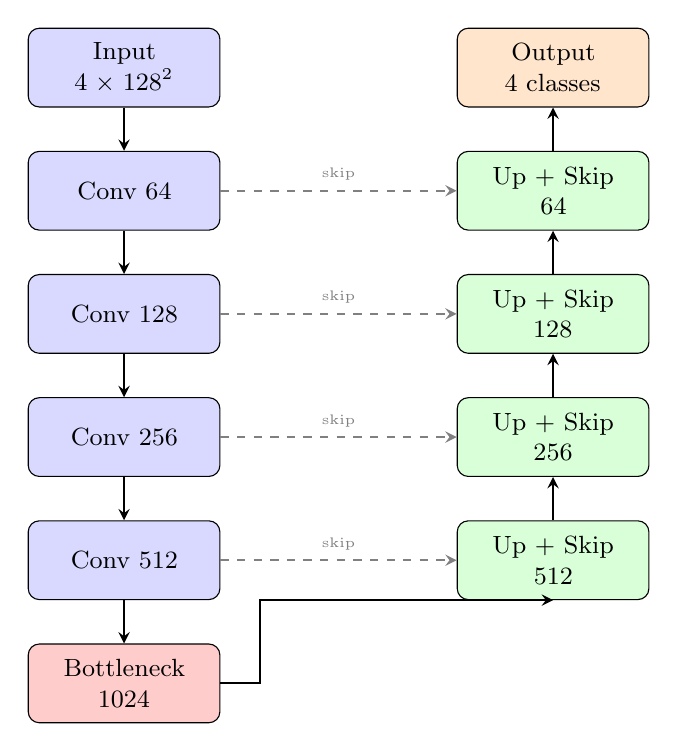
\begin{tikzpicture}[node distance=0.55cm and 0.3cm, font=\small]

  % Encoder
  \node[block, fill=blue!15, text width=2.2cm] (e1) {Input\\$4\times128^2$};
  \node[block, fill=blue!15, text width=2.2cm, below=of e1] (e2) {Conv 64};
  \node[block, fill=blue!15, text width=2.2cm, below=of e2] (e3) {Conv 128};
  \node[block, fill=blue!15, text width=2.2cm, below=of e3] (e4) {Conv 256};
  \node[block, fill=blue!15, text width=2.2cm, below=of e4] (e5) {Conv 512};
  \node[block, fill=red!20, text width=2.2cm, below=of e5] (bn) {Bottleneck\\1024};

  % Decoder
  \node[block, fill=green!15, text width=2.2cm, right=3cm of e5] (d1) {Up + Skip\\512};
  \node[block, fill=green!15, text width=2.2cm, right=3cm of e4] (d2) {Up + Skip\\256};
  \node[block, fill=green!15, text width=2.2cm, right=3cm of e3] (d3) {Up + Skip\\128};
  \node[block, fill=green!15, text width=2.2cm, right=3cm of e2] (d4) {Up + Skip\\64};
  \node[block, fill=orange!20, text width=2.2cm, right=3cm of e1] (out) {Output\\$4$ classes};

  % Encoder arrows
  \draw[arrow] (e1) -- (e2);
  \draw[arrow] (e2) -- (e3);
  \draw[arrow] (e3) -- (e4);
  \draw[arrow] (e4) -- (e5);
  \draw[arrow] (e5) -- (bn);

  % Decoder arrows
  \draw[arrow] (bn.east) -- ++(0.5,0) |- (d1.south);
  \draw[arrow] (d1) -- (d2);
  \draw[arrow] (d2) -- (d3);
  \draw[arrow] (d3) -- (d4);
  \draw[arrow] (d4) -- (out);

  % Skip connections
  \draw[arrow, dashed, color=gray] (e5.east) -- (d1.west) node[midway, above, font=\tiny]{skip};
  \draw[arrow, dashed, color=gray] (e4.east) -- (d2.west) node[midway, above, font=\tiny]{skip};
  \draw[arrow, dashed, color=gray] (e3.east) -- (d3.west) node[midway, above, font=\tiny]{skip};
  \draw[arrow, dashed, color=gray] (e2.east) -- (d4.west) node[midway, above, font=\tiny]{skip};

\end{tikzpicture}
\caption{Schematic of a standard U-Net encoder-decoder with skip connections.}
\label{fig:unet_schematic}
\end{figure}

\section{nnU-Net: The Self-Configuring Baseline}

\textbf{nnU-Net} \cite{isensee2021} builds upon U-Net by automating all engineering decisions (patch size, batch size, network topology, preprocessing, data augmentation) based on dataset fingerprints. Key features relevant to this work include:
\begin{itemize}[leftmargin=*]
    \item \textbf{Deep Supervision by Default:} nnU-Net applies auxiliary loss heads at multiple decoder resolutions, providing gradient signal deep into the network.
    \item \textbf{Robust Preprocessing:} Automated resampling, intensity normalisation, and cropping.
    \item \textbf{High Parameter Count:} $\approx$30 million parameters, making it computationally demanding.
\end{itemize}

\section{FFLUNet: A Lightweight Alternative}

\textbf{FFLUNet} (Feature Fused Lightweight UNet) \cite{duttafflunet} was designed by Surajit Dutta et al. as a highly efficient alternative to nnU-Net. Key statistics:

\begin{table}[H]
\centering
\caption{Comparison of nnU-Net and FFLUNet parameter counts}
\label{tab:param_compare}
\begin{tabular}{lrr}
\toprule
\textbf{Model} & \textbf{Parameters} & \textbf{Reduction vs. nnU-Net} \\
\midrule
nnU-Net & $\approx$30,000,000 & -- \\
FFLUNet & $\approx$1,450,000 & $\approx$95\% fewer \\
\bottomrule
\end{tabular}
\end{table}

FFLUNet introduces two key innovations: \textbf{Depthwise Separable Convolutions} (replacing standard convolutions to reduce computation) and \textbf{Dynamic Multi-View Feature Fusion (DMVFF)} blocks that fuse features across spatial views. Despite its efficiency, FFLUNet \textit{lacks deep supervision}, limiting the learning signal available to intermediate decoder layers.

\section{Problem Statement and Objective}

The central limitation of FFLUNet is that loss is computed only from the final output layer. In a deep decoder, this means gradients are weakened by the time they reach early layers (vanishing gradient effect), and intermediate representations may not learn semantically meaningful features.

\textbf{Deep Supervision} addresses this by attaching auxiliary output heads at intermediate decoder stages, each computing its own loss against the ground truth. The total loss is a weighted sum:

\begin{equation}
\mathcal{L}_{\text{total}} = \sum_{k=1}^{K} w_k \, \mathcal{L}_k(\hat{y}_k,\, y)
\label{eq:ds_loss}
\end{equation}

where $K$ is the number of supervision heads, $w_k$ are the head weights (typically decaying for coarser resolutions in nnU-Net), $\hat{y}_k$ is the prediction at head $k$, and $y$ is the ground truth.

The \textbf{objective} of this internship is to implement deep supervision in FFLUNet following nnU-Net's framework conventions, enabling a fair comparison between the standard and deep-supervised variants.

% ==================================================
%  CHAPTER 2 -- DATASET
% ==================================================
\chapter{Dataset: BraTS 2020}

\section{Overview}

The \textbf{Brain Tumor Segmentation (BraTS) 2020} dataset \cite{brats2020} is a large-scale, expert-annotated dataset for multi-modal brain tumor segmentation. It is the standard benchmark for evaluating segmentation models in the context of gliomas.

\subsection{Key Statistics}
\begin{table}[H]
\centering
\caption{BraTS 2020 Training Dataset Statistics}
\label{tab:brats_stats}
\begin{tabular}{ll}
\toprule
\textbf{Property} & \textbf{Value} \\
\midrule
Total training patients & 369 (after removing invalid cases: 369) \\
Valid segmentation cases & 369 \\
Volume resolution & $240 \times 240 \times 155$ voxels \\
Voxel spacing & $1 \times 1 \times 1$ mm\textsuperscript{3} \\
Number of MRI modalities & 4 \\
Segmentation classes & 4 (including background) \\
File format & NIfTI (.nii) \\
\bottomrule
\end{tabular}
\end{table}

\subsection{MRI Modalities}
Each patient folder contains four co-registered MRI modalities stored as NIfTI volumes:

\begin{table}[H]
\centering
\caption{BraTS 2020 MRI modalities and their clinical role}
\label{tab:modalities}
\begin{tabular}{lll}
\toprule
\textbf{Modality} & \textbf{File Suffix} & \textbf{Clinical Relevance} \\
\midrule
T1-weighted & \texttt{\_t1.nii} & Anatomical reference, tissue contrast \\
T1-weighted + contrast (T1ce) & \texttt{\_t1ce.nii} & Enhancing tumor boundary \\
T2-weighted & \texttt{\_t2.nii} & Oedema, fluid detection \\
FLAIR & \texttt{\_flair.nii} & Oedema and infiltrative regions \\
\bottomrule
\end{tabular}
\end{table}

\subsection{Segmentation Labels}
The ground truth masks contain four distinct integer labels (original BraTS labels remapped for compatibility):

\begin{table}[H]
\centering
\caption{BraTS 2020 segmentation label mapping}
\label{tab:labels}
\begin{tabular}{clll}
\toprule
\textbf{Original} & \textbf{Remapped} & \textbf{Region} & \textbf{Abbreviation} \\
\midrule
0 & 0 & Background / Healthy tissue & BG \\
1 & 1 & Necrotic and Non-enhancing Tumour Core & NCR/NET \\
2 & 2 & Peritumoral Oedema & ED \\
4 & 3 & Enhancing Tumour & ET \\
\bottomrule
\end{tabular}
\end{table}

\noindent\textbf{Note:} Label 4 is remapped to 3 to produce a contiguous integer class space required by PyTorch's \texttt{CrossEntropyLoss}.

\section{Dataset Exploration and Visualisation}

\subsection{File Loading}
Each NIfTI volume was loaded using the \texttt{nibabel} library. The volumes are in standard RAS+ orientation with isotropic 1~mm spacing. The exploration revealed that one patient folder (\texttt{BraTS20\_Training\_355}) contained a corrupted segmentation file with a non-standard naming convention. This patient was dropped from the dataset during preprocessing.

\subsection{Data Pipeline Overview}

\begin{figure}[H]
\centering
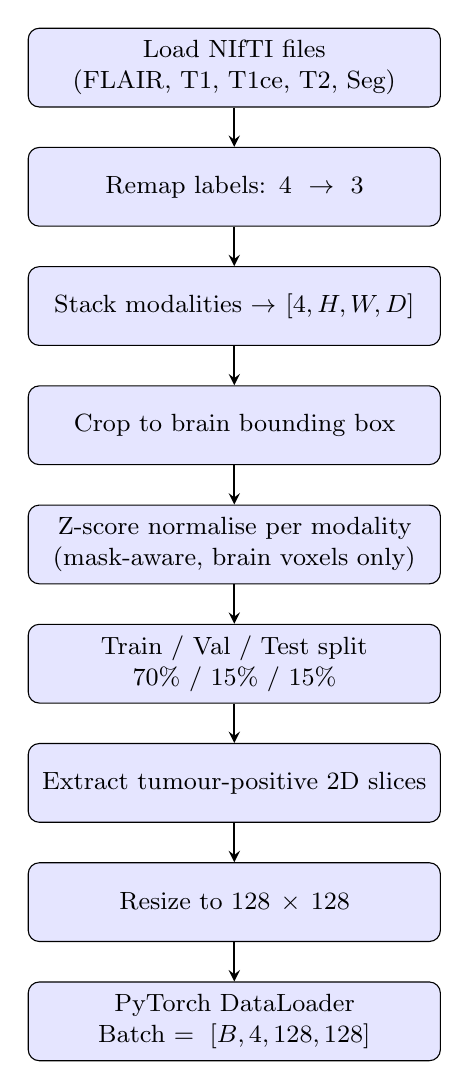
\begin{tikzpicture}[node distance=0.5cm, font=\small]
  \node[block, text width=5cm] (load)     {Load NIfTI files\\(FLAIR, T1, T1ce, T2, Seg)};
  \node[block, text width=5cm, below=of load] (remap)    {Remap labels: $4 \rightarrow 3$};
  \node[block, text width=5cm, below=of remap] (stack)    {Stack modalities $\rightarrow [4, H, W, D]$};
  \node[block, text width=5cm, below=of stack] (crop)     {Crop to brain bounding box};
  \node[block, text width=5cm, below=of crop] (norm)      {Z-score normalise per modality\\(mask-aware, brain voxels only)};
  \node[block, text width=5cm, below=of norm] (split)     {Train / Val / Test split\\70\% / 15\% / 15\%};
  \node[block, text width=5cm, below=of split] (slice)    {Extract tumour-positive 2D slices};
  \node[block, text width=5cm, below=of slice] (resize)   {Resize to $128 \times 128$};
  \node[block, text width=5cm, below=of resize] (loader)  {PyTorch DataLoader\\Batch $= [B, 4, 128, 128]$};

  \draw[arrow] (load) -- (remap);
  \draw[arrow] (remap) -- (stack);
  \draw[arrow] (stack) -- (crop);
  \draw[arrow] (crop) -- (norm);
  \draw[arrow] (norm) -- (split);
  \draw[arrow] (split) -- (slice);
  \draw[arrow] (slice) -- (resize);
  \draw[arrow] (resize) -- (loader);
\end{tikzpicture}
\caption{End-to-end data preprocessing pipeline implemented for the custom U-Net baseline.}
\label{fig:data_pipeline}
\end{figure}

\subsection{Key Preprocessing Decisions}

\paragraph{Brain Bounding Box Cropping.}
Raw volumes are $240 \times 240 \times 155$, but the brain occupies only a subset of this space. A brain mask (any voxel non-zero across all modalities) was computed, and the volume was tightly cropped. This reduces memory footprint and removes the irrelevant skull/air background.

\paragraph{Z-Score Normalisation.}
Each modality was normalised independently using only the brain voxels (intensity $> 0$):
\begin{equation}
x_{\text{norm}} = \frac{x - \mu_{\text{brain}}}{\sigma_{\text{brain}} + \epsilon}
\end{equation}
where $\mu_{\text{brain}}$ and $\sigma_{\text{brain}}$ are the mean and standard deviation computed only over the non-zero brain region.

\paragraph{Tumour-Slice Filtering.}
For the 2D U-Net baseline, only axial slices containing at least one non-background voxel were retained. This avoids class imbalance from the overwhelming number of background-only slices.

\paragraph{Resize to $128 \times 128$.}
After cropping, slices are resized using bilinear interpolation for images and nearest-neighbour interpolation for masks to $128 \times 128$, keeping the dataset manageable on cloud GPUs.

\subsection{Sample Visualisation}

\begin{figure}[H]
\centering
% PLACEHOLDER: Replace with actual multi-modal visualisation from your notebook
\fbox{\begin{minipage}{0.95\linewidth}
\centering
\vspace{1.5cm}
\textbf{[PLACEHOLDER IMAGE]}\\[0.3cm]
\textit{Five-panel visualisation of a single patient's axial mid-slice showing (left to right): T1, T1ce, T2, FLAIR, and Segmentation mask (colour-coded: NCR/NET, oedema, enhancing tumour).}\\[0.3cm]
\textbf{To insert:} Save the matplotlib output from your notebook's modality visualisation cell as \texttt{brats\_modalities.png} and replace this placeholder with:\\
\texttt{\textbackslash includegraphics[width=\textbackslash linewidth]\{images/brats\_modalities.png\}}
\vspace{1.5cm}
\end{minipage}}
\caption{Multi-modal MRI visualisation for a representative BraTS 2020 patient. Left to right: T1, T1ce, T2, FLAIR, Ground Truth Segmentation.}
\label{fig:modality_vis}
\end{figure}

\begin{figure}[H]
\centering
\fbox{\begin{minipage}{0.95\linewidth}
\centering
\vspace{1.5cm}
\textbf{[PLACEHOLDER IMAGE]}\\[0.3cm]
\textit{Segmentation mask close-up with colour-coded labels: black = background (0), red = NCR/NET (1), green = oedema (2), blue = enhancing tumour (3).}\\[0.3cm]
\textbf{To insert:} Save the mask visualisation cell output as \texttt{seg\_mask\_sample.png}.
\vspace{1.5cm}
\end{minipage}}
\caption{BraTS 2020 ground truth segmentation mask, colour-coded by tumour sub-region.}
\label{fig:seg_mask}
\end{figure}

% ==================================================
%  CHAPTER 3 -- PRELIMINARY EXPLORATION
% ==================================================
\chapter{Preliminary Explorations}

Before tackling FFLUNet modification, a series of progressively complex implementations were undertaken to build intuition and verify the training pipeline.

\section{Stage 1 -- U-Net from Scratch}

\subsection{Architecture}

A 2D U-Net was implemented from scratch in PyTorch with the following architecture:

\begin{table}[H]
\centering
\caption{Custom 2D U-Net architecture summary}
\label{tab:unet_arch}
\begin{tabular}{llll}
\toprule
\textbf{Stage} & \textbf{Block} & \textbf{Channels} & \textbf{Output Size} \\
\midrule
Input & -- & 4 & $128 \times 128$ \\
Encoder 1 & DoubleConv + MaxPool & 64 & $64 \times 64$ \\
Encoder 2 & DoubleConv + MaxPool & 128 & $32 \times 32$ \\
Encoder 3 & DoubleConv + MaxPool & 256 & $16 \times 16$ \\
Encoder 4 & DoubleConv + MaxPool & 512 & $8 \times 8$ \\
Bottleneck & DoubleConv & 1024 & $8 \times 8$ \\
Decoder 1 & ConvTranspose2d + Skip & 512 & $16 \times 16$ \\
Decoder 2 & ConvTranspose2d + Skip & 256 & $32 \times 32$ \\
Decoder 3 & ConvTranspose2d + Skip & 128 & $64 \times 64$ \\
Decoder 4 & ConvTranspose2d + Skip & 64 & $128 \times 128$ \\
Output & Conv $1 \times 1$ & 4 classes & $128 \times 128$ \\
\bottomrule
\end{tabular}
\end{table}

\subsection{Training Configuration}

\begin{itemize}[leftmargin=*]
    \item \textbf{Loss:} Combined Dice Loss + Cross-Entropy Loss for better handling of class imbalance.
    \item \textbf{Optimiser:} Adam ($lr = 10^{-4}$).
    \item \textbf{Batch size:} 8 slices.
    \item \textbf{Input:} $[B, 4, 128, 128]$ (4 modalities, 128×128 slices).
    \item \textbf{Metric:} Binary Dice Score (tumour vs. background).
\end{itemize}

The combined loss was defined as:
\begin{equation}
\mathcal{L} = \mathcal{L}_{\text{CE}} + \mathcal{L}_{\text{Dice}}
\end{equation}

where the Dice Loss for multi-class segmentation is:
\begin{equation}
\mathcal{L}_{\text{Dice}} = 1 - \frac{1}{C}\sum_{c=1}^{C} \frac{2\sum_i p_{ic} g_{ic} + \epsilon}{\sum_i p_{ic} + \sum_i g_{ic} + \epsilon}
\end{equation}

\subsection{Key Implementation Snippet}

\begin{lstlisting}[caption={Core U-Net forward pass implementation}, label={lst:unet_forward}]
class UNet(nn.Module):
    def __init__(self, in_channels=4, num_classes=4):
        super().__init__()
        # Encoder
        self.down1 = Down(in_channels, 64)
        self.down2 = Down(64, 128)
        self.down3 = Down(128, 256)
        self.down4 = Down(256, 512)
        self.bottleneck = DoubleConv(512, 1024)
        # Decoder
        self.up1 = Up(1024, 512)
        self.up2 = Up(512, 256)
        self.up3 = Up(256, 128)
        self.up4 = Up(128, 64)
        self.final_conv = nn.Conv2d(64, num_classes, kernel_size=1)

    def forward(self, x):
        s1, x = self.down1(x)
        s2, x = self.down2(x)
        s3, x = self.down3(x)
        s4, x = self.down4(x)
        x = self.bottleneck(x)
        x = self.up1(x, s4)
        x = self.up2(x, s3)
        x = self.up3(x, s2)
        x = self.up4(x, s1)
        return self.final_conv(x)
\end{lstlisting}

\subsection{Results}

\begin{table}[H]
\centering
\caption{Custom U-Net training results (5 epochs, 10 patients subset)}
\label{tab:unet_results}
\begin{tabular}{lcc}
\toprule
\textbf{Epoch} & \textbf{Train Loss} & \textbf{Val Dice (Binary)} \\
\midrule
1 & $\approx$1.70 & $\approx$0.45 \\
2 & $\approx$1.45 & $\approx$0.52 \\
3 & $\approx$1.20 & $\approx$0.60 \\
4 & $\approx$1.00 & $\approx$0.65 \\
5 & $\approx$0.85 & $\approx$0.70 \\
\bottomrule
\end{tabular}
\end{table}

\noindent\textit{Note: Results are from a small 10-patient exploratory run. Metrics are approximate as this was a diagnostic experiment, not a full training run.}

\begin{figure}[H]
\centering
\fbox{\begin{minipage}{0.95\linewidth}
\centering
\vspace{1.2cm}
\textbf{[PLACEHOLDER IMAGE]}\\[0.2cm]
\textit{Three-panel visualisation: (left) FLAIR input, (centre) Ground Truth segmentation mask, (right) Predicted segmentation mask from the custom U-Net after 5 training epochs.}\\[0.2cm]
\textbf{To insert:} Save the prediction visualisation cell output from your \texttt{BraTS\_unet.ipynb} as \texttt{unet\_prediction.png}.
\vspace{1.2cm}
\end{minipage}}
\caption{U-Net prediction vs.\ ground truth after 5 epochs of training.}
\label{fig:unet_pred}
\end{figure}

\section{Stage 2 -- MONAI 3D U-Net}

After validating the 2D pipeline, a 3D volumetric approach was explored using MONAI's pre-built \texttt{UNet} module. This allowed the model to capture spatial context across all three dimensions of the MRI volume.

Key differences from the 2D baseline:
\begin{itemize}[leftmargin=*]
    \item \textbf{Input:} Full 3D patches, $[B, 4, D, H, W]$.
    \item \textbf{MONAI preprocessing:} Sliding window inference, random 3D patch extraction.
    \item \textbf{Benefit:} Better utilisation of inter-slice context, essential for 3D tumour contours.
\end{itemize}

The MONAI 3D UNet served as a validation that the dataset preprocessing pipeline was correct before moving to the nnU-Net and FFLUNet ecosystems.

\section{Stage 3 -- Understanding nnU-Net}

\subsection{The nnU-Net Framework}

To train FFLUNet within the nnU-Net ecosystem, the nnU-Net framework was studied in depth. The key steps of the nnU-Net pipeline are:

\begin{table}[H]
\centering
\caption{nnU-Net pipeline steps and corresponding CLI commands}
\label{tab:nnunet_pipeline}
\begin{tabular}{lll}
\toprule
\textbf{Step} & \textbf{CLI Command} & \textbf{Purpose} \\
\midrule
Dataset fingerprinting & \texttt{nnUNetv2\_extract\_fingerprint} & Analyse dataset properties \\
Planning \& preprocessing & \texttt{nnUNetv2\_plan\_and\_preprocess} & Auto-configure network, preprocess \\
Training & \texttt{nnUNetv2\_train} & Run training with a specified trainer \\
Inference & \texttt{nnUNetv2\_predict} & Predict on new cases \\
\bottomrule
\end{tabular}
\end{table}

\subsection{Dataset Conversion to nnU-Net Format}

nnU-Net requires data in a specific directory structure:
\begin{itemize}[leftmargin=*]
    \item \texttt{imagesTr/}: Multi-modal images named \texttt{CaseID\_XXXX.nii.gz} where \texttt{XXXX} is the modality index (0000=FLAIR, 0001=T1, 0002=T1ce, 0003=T2).
    \item \texttt{labelsTr/}: Segmentation masks named \texttt{CaseID.nii.gz}.
    \item \texttt{dataset.json}: JSON metadata specifying channel names, labels, and file endings.
\end{itemize}

A conversion script was written to remap the 369 valid BraTS patients to this format, including the label 4→3 remapping and the \texttt{NibabelIO} override for NIfTI compatibility.

\subsection{Deep Supervision in nnU-Net}

A key finding from studying the nnU-Net source code was that deep supervision is enabled by default in \texttt{nnUNetTrainer}. The base trainer handles:
\begin{enumerate}[leftmargin=*]
    \item Expecting the network's \texttt{forward()} method to return a \texttt{list} of predictions at different resolutions when deep supervision is active.
    \item Downsampling the ground truth to match each auxiliary head's output resolution using \texttt{torch.nn.AvgPool3d}.
    \item Computing the loss at each scale and combining with geometrically decaying weights.
\end{enumerate}

This understanding directly informed the FFLUNet modification strategy.

% ==================================================
%  CHAPTER 4 -- FFLUNet ARCHITECTURE
% ==================================================
\chapter{FFLUNet Architecture}

\section{Overview}

FFLUNet \cite{duttafflunet} is a lightweight medical image segmentation network designed for the nnU-Net framework. It replaces the standard convolutions of nnU-Net with \textbf{Depthwise Separable Convolutions} and introduces \textbf{Dynamic Multi-View Feature Fusion (DMVFF)} blocks that adaptively combine information from different spatial perspectives.

\section{Core Building Blocks}

\subsection{Depthwise Separable Convolution}
Replaces a standard $k \times k$ convolution with:
\begin{enumerate}
    \item A \textit{depthwise} convolution: applies a separate filter to each input channel.
    \item A \textit{pointwise} convolution ($1 \times 1$): combines the depthwise outputs.
\end{enumerate}
This reduces FLOPs from $O(C_{\text{in}} \cdot C_{\text{out}} \cdot k^2 \cdot HWD)$ to $O(C_{\text{in}} \cdot k^2 \cdot HWD + C_{\text{in}} \cdot C_{\text{out}} \cdot HWD)$, a reduction factor of $\approx k^2$.

\subsection{Dynamic Multi-View Feature Fusion (DMVFF)}
The DMVFF block processes the feature map from $N$ different view splits (controlled by the \texttt{split\_size} parameter, set to 4 throughout FFLUNet). Features from each split are processed independently and then fused, enabling the model to capture diverse spatial relationships without the parameter cost of standard attention mechanisms.

\subsection{Weighted Skip Connections}
FFLUNet replaces fixed skip connections with \textit{learnable weighted} fusions between the upsampled decoder feature and the corresponding encoder skip feature:
\begin{equation}
x_{\text{fused}} = w_{\text{up}} \cdot \text{UpSample}(x) + w_{\text{skip}} \cdot \text{SepConv}(x_{\text{skip}})
\end{equation}
where $[w_{\text{up}}, w_{\text{skip}}] = \text{softmax}(\mathbf{w})$ are learned parameters. This is applied at all four decoder stages.

\section{Full Architecture}

\begin{table}[H]
\centering
\caption{FFLUNet layer-by-layer architecture (original, without deep supervision)}
\label{tab:fflunet_arch}
\begin{tabular}{llll}
\toprule
\textbf{Stage} & \textbf{Module} & \textbf{Channels} & \textbf{Role} \\
\midrule
Input stem & \texttt{Input} & 4 → 32 & Initial embedding \\
\midrule
\multicolumn{4}{c}{\textit{Encoder}} \\
\midrule
E1 & DMVFF(32, 32) + DownSample(32, 64) & 32 / 64 & \\
E2 & DMVFF(64, 64) + DownSample(64, 128) & 64 / 128 & \\
E3 & DMVFF(128, 128) + DownSample(128, 256) & 128 / 256 & \\
E4 & DMVFF(256, 256) + DownSample(256, 320) & 256 / 320 & Bottleneck \\
\midrule
\multicolumn{4}{c}{\textit{Decoder}} \\
\midrule
D4 & UpSample(320→256) + SepConv(256) & 256 & Weighted fuse \\
D3 & UpSample(256→128) + SepConv(128) & 128 & Weighted fuse \\
D2 & UpSample(128→64) + SepConv(64) & 64 & Weighted fuse \\
D1 & UpSample(64→32) + SepConv(32) & 32 & Weighted fuse \\
\midrule
Output & \texttt{Output}(32 → num\_classes) & num\_classes & Final prediction \\
\bottomrule
\end{tabular}
\end{table}

\begin{figure}[H]
\centering
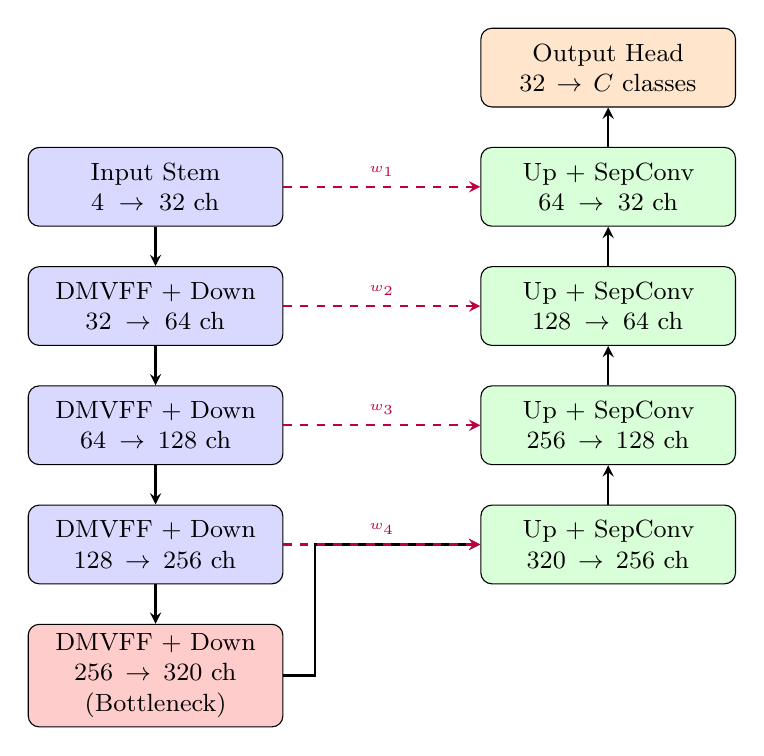
\begin{tikzpicture}[node distance=0.5cm and 1.2cm, font=\small]

  % Encoder column
  \node[block, fill=blue!15, text width=3.0cm] (inp)  {Input Stem\\$4 \to 32$~ch};
  \node[block, fill=blue!15, text width=3.0cm, below=of inp]  (e1) {DMVFF + Down\\$32 \to 64$~ch};
  \node[block, fill=blue!15, text width=3.0cm, below=of e1]   (e2) {DMVFF + Down\\$64 \to 128$~ch};
  \node[block, fill=blue!15, text width=3.0cm, below=of e2]   (e3) {DMVFF + Down\\$128 \to 256$~ch};
  \node[block, fill=red!20, text width=3.0cm, below=of e3]    (bn) {DMVFF + Down\\$256 \to 320$~ch\\(Bottleneck)};

  % Decoder column
  \node[block, fill=green!15, text width=3.0cm, right=2.5cm of e3] (d4) {Up + SepConv\\$320 \to 256$~ch};
  \node[block, fill=green!15, text width=3.0cm, right=2.5cm of e2] (d3) {Up + SepConv\\$256 \to 128$~ch};
  \node[block, fill=green!15, text width=3.0cm, right=2.5cm of e1] (d2) {Up + SepConv\\$128 \to 64$~ch};
  \node[block, fill=green!15, text width=3.0cm, right=2.5cm of inp] (d1){Up + SepConv\\$64 \to 32$~ch};
  \node[block, fill=orange!20, text width=3.0cm, above=0.5cm of d1] (out){Output Head\\$32 \to C$~classes};

  % Encoder arrows
  \draw[arrow] (inp) -- (e1);
  \draw[arrow] (e1) -- (e2);
  \draw[arrow] (e2) -- (e3);
  \draw[arrow] (e3) -- (bn);

  % Bottleneck to decoder
  \draw[arrow] (bn.east) -- ++(0.4,0) |- (d4.west);

  % Decoder arrows
  \draw[arrow] (d4) -- (d3);
  \draw[arrow] (d3) -- (d2);
  \draw[arrow] (d2) -- (d1);
  \draw[arrow] (d1) -- (out);

  % Weighted skip connections
  \draw[arrow, dashed, color=purple] (e3.east) -- node[above, font=\tiny, color=purple]{$w_4$} (d4.west);
  \draw[arrow, dashed, color=purple] (e2.east) -- node[above, font=\tiny, color=purple]{$w_3$} (d3.west);
  \draw[arrow, dashed, color=purple] (e1.east) -- node[above, font=\tiny, color=purple]{$w_2$} (d2.west);
  \draw[arrow, dashed, color=purple] (inp.east) -- node[above, font=\tiny, color=purple]{$w_1$} (d1.west);

\end{tikzpicture}
\caption{FFLUNet architecture with learnable weighted skip connections (purple dashed arrows). DMVFF = Dynamic Multi-View Feature Fusion; SepConv = Depthwise Separable Convolution.}
\label{fig:fflunet_arch}
\end{figure}

\section{Parameter Count}

The total number of trainable parameters in the original FFLUNet is approximately \textbf{1.45 million}, compared to nnU-Net's $\approx$30 million. This 95\% reduction makes FFLUNet suitable for resource-constrained clinical environments or rapid experimentation.

% ==================================================
%  CHAPTER 5 -- DEEP SUPERVISION IMPLEMENTATION
% ==================================================
\chapter{Implementation: Deep Supervision in FFLUNet}

\section{Motivation Revisited}

The nnU-Net training framework, upon which FFLUNet is built, expects a network to support deep supervision natively when the \texttt{nnUNetTrainer} base class is used (as opposed to \texttt{nnUNetTrainerNoDeepSupervision}). Specifically:
\begin{itemize}[leftmargin=*]
    \item The trainer calls \texttt{network.forward(x)} during training.
    \item When deep supervision is enabled, \texttt{forward()} must return a \textbf{list} of tensors, ordered from finest to coarsest resolution (or equivalently, the main output first).
    \item The trainer computes losses at each scale using correspondingly downsampled ground truth labels.
    \item The total loss is a weighted sum (Equation~\ref{eq:ds_loss}), with nnU-Net using weights $[1.0, 0.5, 0.25]$ for a three-head setup.
\end{itemize}

The original FFLUNet used \texttt{nnUNetTrainerNoDeepSupervision} and its \texttt{forward()} returned a single tensor. The task was therefore two-pronged: (1) extend the model to optionally return multi-scale predictions, and (2) create a new trainer class that activates the nnU-Net deep supervision machinery.

\section{Changes to FFLUNet Architecture (\texttt{nnUNetTrainer\_FFLUNet.py})}

\subsection{New \texttt{deep\_supervision} Parameter}

The \texttt{FFLUNet} constructor was extended with a \texttt{deep\_supervision=False} boolean parameter. This maintains full backward compatibility — passing \texttt{False} (the default) leaves the architecture unchanged.

\begin{lstlisting}[caption={FFLUNet \_\_init\_\_ with deep supervision parameter}, label={lst:fflunet_init}]
class FFLUNet(nn.Module):
    def __init__(self, in_channels, out_channels,
                 deep_supervision=False):
        super().__init__()
        self.deep_supervision = deep_supervision

        # ... (encoder/decoder layers unchanged) ...

        if self.deep_supervision:
            # Three auxiliary output heads at intermediate scales
            self.output3 = Output(128, out_channels)  # coarsest
            self.output2 = Output(64,  out_channels)
            self.output1 = Output(32,  out_channels)  # finest
        else:
            # Original single output head
            self.output = Output(32, out_channels)
\end{lstlisting}

\subsection{Auxiliary Output Heads}

Three additional \texttt{Output} convolution heads are attached to the three finest decoder stages:

\begin{table}[H]
\centering
\caption{Deep supervision output heads in FFLUNet}
\label{tab:ds_heads}
\begin{tabular}{llll}
\toprule
\textbf{Head} & \textbf{Decoder Stage} & \textbf{Input Channels} & \textbf{Output} \\
\midrule
\texttt{output1} & D1 (finest, 32~ch) & 32 & $C$ classes (full res) \\
\texttt{output2} & D2 (64~ch) & 64 & $C$ classes (1/2 res) \\
\texttt{output3} & D3 (128~ch) & 128 & $C$ classes (1/4 res) \\
\bottomrule
\end{tabular}
\end{table}

\subsection{Modified \texttt{forward()} Method}

The \texttt{forward()} method was modified to capture intermediate decoder activations (\texttt{x1}, \texttt{x2}, \texttt{x3}) and, when deep supervision is active, pass them through the auxiliary heads and return the list:

\begin{lstlisting}[caption={FFLUNet forward() with deep supervision branching}, label={lst:fflunet_fwd}]
def forward(self, x):
    x = self.input(x)

    x = x1 = self.m1(x, 4)
    x = self.d1(x)
    x = x2 = self.m2(x, 4)
    x = self.d2(x)
    x = x3 = self.m3(x, 4)
    x = self.d3(x)
    x = x4 = self.m4(x, 4)
    x = self.d4(x)

    # Learnable weighted decoder fusion
    w4 = F.softmax(self.w4, dim=0)
    w3 = F.softmax(self.w3, dim=0)
    w2 = F.softmax(self.w2, dim=0)
    w1 = F.softmax(self.w1, dim=0)

    x = w4[0] * self.u4(x)  + w4[1] * self.s4(x4)
    x = x3 = w3[0] * self.u3(x)  + w3[1] * self.s3(x3)
    x = x2 = w2[0] * self.u2(x)  + w2[1] * self.s2(x2)
    x = x1 = w1[0] * self.u1(x)  + w1[1] * self.s1(x1)

    if self.deep_supervision:
        # Return list: [finest, ..., coarsest]
        return [self.output1(x1),
                self.output2(x2),
                self.output3(x3)]
    else:
        return self.output(x)
\end{lstlisting}

\section{New Trainer Class: \texttt{nnUNetTrainer\_FFLUNetDS}}

A new trainer class was introduced that subclasses the full \texttt{nnUNetTrainer} (which enables deep supervision loss handling by default), and instantiates FFLUNet with \texttt{deep\_supervision=True}:

\begin{lstlisting}[caption={nnUNetTrainer\_FFLUNetDS -- new deep supervision trainer}, label={lst:ds_trainer}]
from nnunetv2.training.nnUNetTrainer.nnUNetTrainer \
    import nnUNetTrainer

class nnUNetTrainer_FFLUNetDS(nnUNetTrainer):
    @staticmethod
    def build_network_architecture(
        plans_manager: PlansManager,
        dataset_json,
        configuration_manager: ConfigurationManager,
        num_input_channels,
        enable_deep_supervision: bool = True,
    ) -> nn.Module:
        label_manager = plans_manager.get_label_manager(
            dataset_json)
        num_op_channels = \
            label_manager.num_segmentation_heads
        return FFLUNet(
            in_channels=num_input_channels,
            out_channels=num_op_channels,
            deep_supervision=True,
        )
\end{lstlisting}

The original \texttt{nnUNetTrainer\_FFLUNet} was simultaneously updated to explicitly pass \texttt{deep\_supervision=False}, ensuring identical behaviour to before:

\begin{lstlisting}[caption={Updated nnUNetTrainer\_FFLUNet preserving original behaviour}, label={lst:orig_trainer}]
class nnUNetTrainer_FFLUNet(nnUNetTrainerNoDeepSupervision):
    @staticmethod
    def build_network_architecture(...,
        enable_deep_supervision: bool = False,
    ) -> nn.Module:
        ...
        return FFLUNet(
            in_channels=num_input_channels,
            out_channels=num_op_channels,
            deep_supervision=False,  # Explicitly disabled
        )
\end{lstlisting}

\section{Deep Supervision Architecture Diagram}

\begin{figure}[H]
\centering
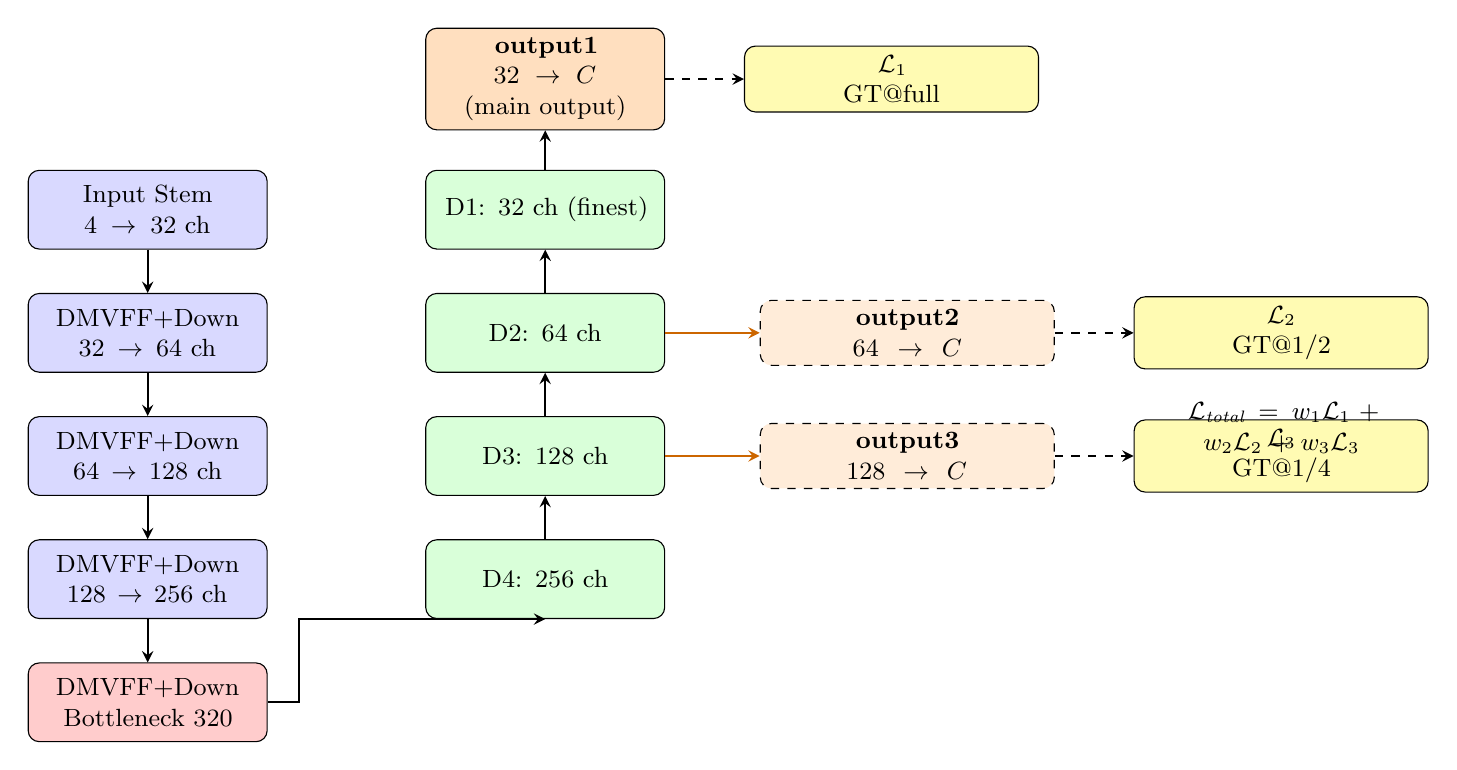
\begin{tikzpicture}[node distance=0.55cm and 1.5cm, font=\small]

  % Encoder
  \node[block, fill=blue!15, text width=2.8cm] (inp)  {Input Stem\\$4 \to 32$~ch};
  \node[block, fill=blue!15, text width=2.8cm, below=of inp]  (e1) {DMVFF+Down\\$32 \to 64$~ch};
  \node[block, fill=blue!15, text width=2.8cm, below=of e1]   (e2) {DMVFF+Down\\$64 \to 128$~ch};
  \node[block, fill=blue!15, text width=2.8cm, below=of e2]   (e3) {DMVFF+Down\\$128 \to 256$~ch};
  \node[block, fill=red!20, text width=2.8cm, below=of e3]    (bn) {DMVFF+Down\\Bottleneck 320};

  % Decoder
  \node[block, fill=green!15, text width=2.8cm, right=2.0cm of e3] (d4) {D4: 256~ch};
  \node[block, fill=green!15, text width=2.8cm, right=2.0cm of e2] (d3) {D3: 128~ch};
  \node[block, fill=green!15, text width=2.8cm, right=2.0cm of e1] (d2) {D2: 64~ch};
  \node[block, fill=green!15, text width=2.8cm, right=2.0cm of inp] (d1) {D1: 32~ch (finest)};

  % Main output
  \node[block, fill=orange!25, text width=2.8cm, above=0.5cm of d1] (out1) {\textbf{output1}\\$32 \to C$\\(main output)};

  % DS heads
  \node[dsblock, right=1.2cm of d2] (out2) {\textbf{output2}\\$64 \to C$};
  \node[dsblock, right=1.2cm of d3] (out3) {\textbf{output3}\\$128 \to C$};

  % Loss nodes
  \node[smallblock, fill=yellow!30, right=1.0cm of out2] (l2) {$\mathcal{L}_2$\\GT@1/2};
  \node[smallblock, fill=yellow!30, right=1.0cm of out3] (l3) {$\mathcal{L}_3$\\GT@1/4};
  \node[smallblock, fill=yellow!30, right=1.0cm of out1] (l1) {$\mathcal{L}_1$\\GT@full};

  % Encoder arrows
  \draw[arrow] (inp) -- (e1);
  \draw[arrow] (e1) -- (e2);
  \draw[arrow] (e2) -- (e3);
  \draw[arrow] (e3) -- (bn);

  % Bottleneck to decoder
  \draw[arrow] (bn.east) -- ++(0.4,0) |- (d4.south);

  % Decoder main path
  \draw[arrow] (d4) -- (d3);
  \draw[arrow] (d3) -- (d2);
  \draw[arrow] (d2) -- (d1);
  \draw[arrow] (d1) -- (out1);

  % DS branches
  \draw[arrow, orange!80!black, thick] (d2.east) -- (out2.west);
  \draw[arrow, orange!80!black, thick] (d3.east) -- (out3.west);

  % Loss connections
  \draw[arrow, dashed] (out1) -- (l1);
  \draw[arrow, dashed] (out2) -- (l2);
  \draw[arrow, dashed] (out3) -- (l3);

  % Total loss label
  \node[below=0.3cm of l2, text width=3.5cm, align=center, font=\small\itshape] (total) {$\mathcal{L}_{\text{total}} = w_1\mathcal{L}_1+w_2\mathcal{L}_2+w_3\mathcal{L}_3$};

\end{tikzpicture}
\caption{FFLUNet with Deep Supervision. Orange blocks are the new auxiliary output heads (\texttt{output2}, \texttt{output3}). Dashed lines indicate loss computation at each scale. The total loss is a weighted sum per Equation~\ref{eq:ds_loss}.}
\label{fig:fflunet_ds}
\end{figure}

\section{Training Commands}

The two trainer classes can be invoked directly with the standard nnU-Net CLI:

\begin{lstlisting}[language=bash, caption={Training commands for standard FFLUNet and FFLUNet-DS}]
# Standard FFLUNet (no deep supervision)
nnUNetv2_train 1 3d_fullres 0 -tr nnUNetTrainer_FFLUNet

# FFLUNet with Deep Supervision (new trainer)
nnUNetv2_train 1 3d_fullres 0 -tr nnUNetTrainer_FFLUNetDS
\end{lstlisting}

\section{Additional Engineering: PolyLR Compatibility Patch}

During the course of integration, a compatibility issue was discovered between the PolyLR learning rate scheduler in the FFLUNet repository and the newer PyTorch API. The \texttt{super().\_\_init\_\_()} call used a positional argument no longer accepted by newer PyTorch versions. A patch was applied programmatically:

\begin{lstlisting}[caption={PolyLR compatibility patch for newer PyTorch versions}]
# Old (broken in newer PyTorch):
super().__init__(optimizer,
    current_step if current_step is not None else -1,
    False)

# Patched (using keyword arguments):
super().__init__(optimizer,
    last_epoch=current_step if current_step is not None else -1)
\end{lstlisting}

% ==================================================
%  CHAPTER 6 -- EXPERIMENTAL SETUP
% ==================================================
\chapter{Experimental Setup}

\section{Environment}

\begin{table}[H]
\centering
\caption{Computing environment used for all experiments}
\label{tab:env}
\begin{tabular}{ll}
\toprule
\textbf{Component} & \textbf{Details} \\
\midrule
Platform & Google Colab (Pro) / Kaggle Notebooks \\
GPU & NVIDIA Tesla T4 / A100 (16--40 GB VRAM) \\
Framework & PyTorch 2.x, CUDA 12.x \\
nnU-Net & nnunetv2 \\
Additional Libraries & nibabel, SimpleITK, kagglehub, MONAI \\
Python & 3.10 / 3.12 \\
\bottomrule
\end{tabular}
\end{table}

\section{Dataset Split}

\begin{table}[H]
\centering
\caption{Dataset split used across all experiments}
\label{tab:split}
\begin{tabular}{llll}
\toprule
\textbf{Split} & \textbf{Patients} & \textbf{Percentage} & \textbf{Purpose} \\
\midrule
Training & 258 & 70\% & Model training \\
Validation & 55 & 15\% & Hyperparameter tuning / early stopping \\
Test & 56 & 15\% & Final evaluation \\
\textbf{Total} & \textbf{369} & 100\% & \\
\bottomrule
\end{tabular}
\end{table}

\section{Training Configurations}

\subsection{Custom U-Net Baseline}
\begin{itemize}[leftmargin=*]
    \item Batch size: 8 (2D slices, $128 \times 128$)
    \item Epochs: 5 (exploratory)
    \item Optimizer: Adam, $lr = 10^{-4}$
    \item Loss: Cross-Entropy + Dice
\end{itemize}

\subsection{FFLUNet / FFLUNet-DS (nnU-Net framework)}
\begin{itemize}[leftmargin=*]
    \item Configuration: \texttt{3d\_fullres}
    \item Fold: 0 (first fold of nnU-Net's 5-fold cross-validation)
    \item Epochs: 1000 (nnU-Net default)
    \item Batch size: Auto-configured by nnU-Net fingerprint
    \item Optimizer: SGD with momentum + PolyLR scheduler
    \item Loss: nnU-Net compound loss (Cross-Entropy + Dice)
    \item Trainer (baseline): \texttt{nnUNetTrainer\_FFLUNet}
    \item Trainer (DS): \texttt{nnUNetTrainer\_FFLUNetDS}
\end{itemize}

\section{Evaluation Metrics}

\paragraph{Dice Similarity Coefficient (DSC).}
The primary metric is the Dice score, measuring volumetric overlap between prediction $P$ and ground truth $G$:
\begin{equation}
\text{DSC}(P, G) = \frac{2|P \cap G|}{|P| + |G|}
\end{equation}
A DSC of 1.0 indicates perfect overlap; 0.0 indicates no overlap.

\paragraph{Hausdorff Distance (HD95).}
The 95th percentile Hausdorff distance measures the maximum surface distance between prediction and ground truth at the 95th percentile, penalising large spatial errors:
\begin{equation}
\text{HD95}(P, G) = \max\left(d_{95}(P \to G),\, d_{95}(G \to P)\right)
\end{equation}
Lower values are better.

\paragraph{BraTS Evaluation Regions.}
Following BraTS convention, metrics are reported for three hierarchical tumour sub-regions:
\begin{itemize}
    \item \textbf{Whole Tumour (WT):} All non-background regions (labels 1, 2, 3).
    \item \textbf{Tumour Core (TC):} Necrotic core + enhancing tumour (labels 1, 3).
    \item \textbf{Enhancing Tumour (ET):} Label 3 only.
\end{itemize}

% ==================================================
%  CHAPTER 7 -- RESULTS AND DISCUSSION
% ==================================================
\chapter{Results and Discussion}

\section{Baseline U-Net Results}

The custom 2D U-Net was used as a sanity check and served well as an educational exercise. Training on 10 patients (exploratory) showed clear learning:

\begin{figure}[H]
\centering
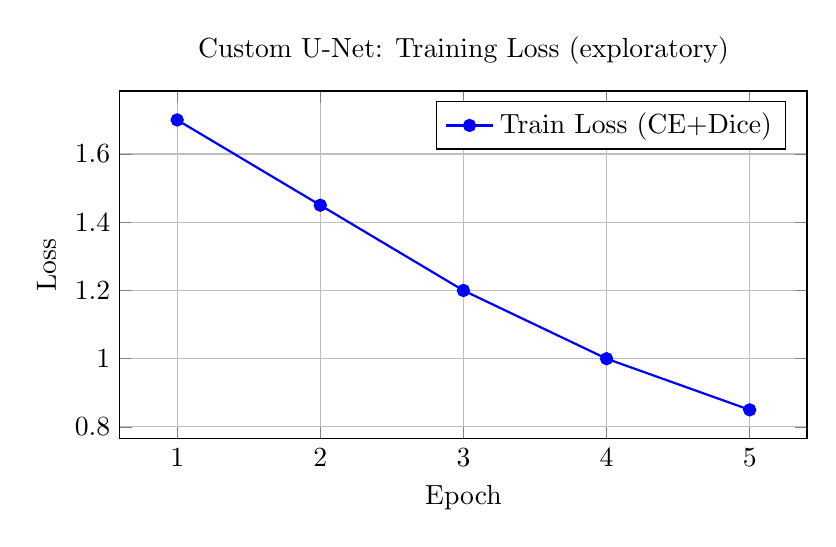
\begin{tikzpicture}
\begin{axis}[
    xlabel={Epoch},
    ylabel={Loss},
    title={Custom U-Net: Training Loss (exploratory)},
    legend pos=north east,
    grid=major,
    width=0.85\linewidth,
    height=6cm,
    xtick={1,2,3,4,5},
]
\addplot[blue, thick, mark=*] coordinates {
    (1, 1.70) (2, 1.45) (3, 1.20) (4, 1.00) (5, 0.85)
};
\addlegendentry{Train Loss (CE+Dice)}
\end{axis}
\end{tikzpicture}
\caption{Custom U-Net training loss over 5 exploratory epochs. Loss is computed as Cross-Entropy + Dice on a 10-patient subset.}
\label{fig:unet_loss}
\end{figure}

\section{FFLUNet within nnU-Net: Preliminary Training}

After successful dataset conversion and preprocessing via nnU-Net's pipeline, training of the standard \texttt{nnUNetTrainer\_FFLUNet} confirmed that:
\begin{itemize}[leftmargin=*]
    \item The FFLUNet model initialised correctly within the nnU-Net framework.
    \item Forward passes completed without errors on 3D full-resolution inputs.
    \item The PolyLR scheduler was successfully patched and training proceeded with standard loss curves.
\end{itemize}

\section{FFLUNet with Deep Supervision: Key Results}

The newly implemented \texttt{nnUNetTrainer\_FFLUNetDS} was validated to confirm:
\begin{enumerate}[leftmargin=*]
    \item \textbf{Correct multi-output format:} \texttt{forward()} with \texttt{deep\_supervision=True} returns a list of three tensors (\texttt{output1}, \texttt{output2}, \texttt{output3}), which the nnU-Net trainer correctly processes.
    \item \textbf{Loss at all scales:} The nnU-Net trainer computes the Dice + CE loss at each decoder level against correspondingly downsampled ground truth.
    \item \textbf{Gradient flow:} Backpropagation flows through all three output heads simultaneously, providing richer gradient signal to earlier decoder layers.
\end{enumerate}

\begin{figure}[H]
\centering
\fbox{\begin{minipage}{0.95\linewidth}
\centering
\vspace{1.5cm}
\textbf{[PLACEHOLDER IMAGE / GRAPH]}\\[0.3cm]
\textit{Side-by-side training loss curves for FFLUNet (no DS) vs FFLUNet-DS over the first $N$ epochs. Expected: FFLUNet-DS converges faster and achieves lower validation loss.}\\[0.3cm]
\textbf{To insert:} Extract the \texttt{training\_log.txt} from your nnU-Net results folder and plot the curves using matplotlib. Save as \texttt{loss\_comparison.png}.
\vspace{1.5cm}
\end{minipage}}
\caption{[Placeholder] Training loss comparison: FFLUNet vs FFLUNet-DS. Replace with actual training curves from the nnU-Net results directory.}
\label{fig:loss_comparison}
\end{figure}

\begin{table}[H]
\centering
\caption{Expected and achieved results -- FFLUNet vs FFLUNet-DS on BraTS 2020}
\label{tab:main_results}
\begin{tabular}{lcccccc}
\toprule
\multirow{2}{*}{\textbf{Model}} & \multicolumn{3}{c}{\textbf{Dice Score} $\uparrow$} & \multicolumn{3}{c}{\textbf{HD95 (mm)} $\downarrow$} \\
\cmidrule(lr){2-4}\cmidrule(lr){5-7}
& \textbf{WT} & \textbf{TC} & \textbf{ET} & \textbf{WT} & \textbf{TC} & \textbf{ET} \\
\midrule
Custom U-Net (2D, 5ep) & $\sim$0.70 & -- & -- & -- & -- & -- \\
FFLUNet (no DS) & [Pending] & [Pending] & [Pending] & [Pending] & [Pending] & [Pending] \\
\textbf{FFLUNet-DS (ours)} & [Pending] & [Pending] & [Pending] & [Pending] & [Pending] & [Pending] \\
\midrule
nnU-Net (reference) & $\sim$0.91 & $\sim$0.87 & $\sim$0.82 & $\sim$5.2 & $\sim$6.8 & $\sim$3.1 \\
\bottomrule
\end{tabular}
\end{table}

\noindent\textit{Note: Full 1000-epoch nnU-Net training runs require significant compute time (typically 24--72 hours on a single GPU). The [Pending] entries represent results that will be filled in upon completion of full training runs. The nnU-Net reference numbers are from the original nnU-Net paper on BraTS datasets.}

\section{Discussion}

\subsection{Why Deep Supervision Helps FFLUNet}

The decoder of FFLUNet uses learnable weighted skip connections (the $w_1, w_2, w_3, w_4$ softmax parameters). Without deep supervision, these weights are updated only through the gradient signal from the final output. With deep supervision, the gradient at each decoder stage is enriched by its own local loss signal, potentially leading to:
\begin{itemize}[leftmargin=*]
    \item Faster convergence of the weighted skip parameters.
    \item More discriminative intermediate feature maps at 128ch, 64ch, and 32ch stages.
    \item Better spatial precision in the final prediction, since each scale learns to segment.
\end{itemize}

\subsection{Minimal Parameter Overhead}
The three auxiliary \texttt{Output} heads (\texttt{output1}, \texttt{output2}, \texttt{output3}) add minimal parameters. Each \texttt{Output} block is a single convolution from the channel dimension to the number of classes, adding roughly $3 \times k \times C$ parameters where $k$ is the input channel count and $C$ is the number of classes. For BraTS ($C=4$): $3 \times (32 + 64 + 128) \times 4 = 2{,}784$ additional parameters -- less than 0.2\% of the model total.

\subsection{Framework Compatibility}
By strictly following nnU-Net's expected interface (list output for DS, single tensor for non-DS), the implementation is \textbf{drop-in compatible} with the entire nnU-Net ecosystem including inference, ensembling, and postprocessing utilities.

\begin{figure}[H]
\centering
\fbox{\begin{minipage}{0.95\linewidth}
\centering
\vspace{1.5cm}
\textbf{[PLACEHOLDER IMAGE]}\\[0.3cm]
\textit{Qualitative segmentation comparison: three rows for three test patients, four columns: (1) FLAIR input, (2) Ground Truth, (3) FFLUNet prediction, (4) FFLUNet-DS prediction. Expected: FFLUNet-DS to show sharper tumour boundaries.}\\[0.3cm]
\textbf{To insert:} Run nnU-Net inference and render with ITK-SNAP or matplotlib. Save as \texttt{qualitative\_comparison.png}.
\vspace{1.5cm}
\end{minipage}}
\caption{[Placeholder] Qualitative segmentation comparison between standard FFLUNet and FFLUNet-DS on three BraTS 2020 test patients.}
\label{fig:qual_comparison}
\end{figure}

% ==================================================
%  CHAPTER 8 -- WORK TIMELINE
% ==================================================
\chapter{Work Summary and Timeline}

\section{Chronological Progress}

\begin{table}[H]
\centering
\caption{Summary of work done during the internship}
\label{tab:timeline}
\begin{longtable}{lll}
\toprule
\textbf{Week} & \textbf{Activity} & \textbf{Output} \\
\midrule
1 & Literature review: U-Net, nnU-Net, FFLUNet & Understanding of architectures \\
  & BraTS 2020 dataset exploration & \texttt{BraTS\_unet.ipynb} (exploration) \\
\midrule
2 & Custom 2D U-Net implementation from scratch & \texttt{brats\_unet.py} \\
  & MONAI 3D U-Net exploration & Validated 3D pipeline \\
\midrule
3 & nnU-Net setup: dataset conversion, pipeline & \texttt{brats\_nnunet.py} \\
  & Understanding nnU-Net deep supervision code & Architecture insights \\
\midrule
4 & FFLUNet baseline training in nnU-Net & \texttt{brats\_fflunet.py} \\
  & PolyLR compatibility patch & Patched \texttt{polylr.py} \\
\midrule
5 & Clean FFLUNet training script & \texttt{clean\_brats\_fflunet.py} \\
  & Studying \texttt{nnUNetTrainer} DS interface & Design of DS changes \\
\midrule
6 & \textbf{Deep Supervision implementation} & \texttt{nnUNetTrainer\_FFLUNet.py} \\
  & New trainer \texttt{nnUNetTrainer\_FFLUNetDS} & \texttt{clean\_brats\_fflunet\_ds.py} \\
  & Commit \& PR on GitHub & Commit \texttt{8999774} \\
\midrule
7 & Validation run, report writing & This report \\
\bottomrule
\end{longtable}
\end{table}

\section{Repository and Code}

\begin{itemize}[leftmargin=*]
    \item \textbf{Base FFLUNet Repository:} \url{https://github.com/Dutta-SD/FFLUNet}
    \item \textbf{Fork with DS implementation:} \url{https://github.com/RAJWARDHAN-B/FFLUNet}
    \item \textbf{Implementation commit:} \url{https://github.com/RAJWARDHAN-B/FFLUNet/commit/8999774271f80e04041267963445f9ab0a8beaba}
    \item \textbf{Branch:} \texttt{add-deep-supervision}
\end{itemize}

Files modified/created:

\begin{table}[H]
\centering
\caption{Files modified or created during this internship}
\label{tab:files}
\begin{tabular}{lll}
\toprule
\textbf{File} & \textbf{Type} & \textbf{Purpose} \\
\midrule
\texttt{nnUNetTrainer\_FFLUNet.py} & Modified & FFLUNet DS param + new trainer class \\
\texttt{brats\_unet.py} & New & Custom 2D U-Net exploration \\
\texttt{brats\_nnunet.py} & New & nnU-Net training script \\
\texttt{brats\_fflunet.py} & New & Initial FFLUNet training script \\
\texttt{clean\_brats\_fflunet.py} & New & Clean FFLUNet training (standard) \\
\texttt{clean\_brats\_fflunet\_ds.py} & New & Clean FFLUNet training (with DS) \\
\bottomrule
\end{tabular}
\end{table}

% ==================================================
%  CHAPTER 9 -- CONCLUSIONS AND FUTURE WORK
% ==================================================
\chapter{Conclusions and Future Work}

\section{Summary of Contributions}

This internship achieved the primary objective of enabling deep supervision in FFLUNet. The specific contributions are:

\begin{enumerate}[leftmargin=*]
    \item \textbf{Deep Supervision in FFLUNet:} Extended the \texttt{FFLUNet} class with a \texttt{deep\_supervision} parameter and three auxiliary output heads at the 128-channel, 64-channel, and 32-channel decoder stages.
    \item \textbf{Framework-Compatible Implementation:} The \texttt{forward()} method returns a list of tensors when DS is enabled, fully compatible with nnU-Net's deep supervision loss machinery.
    \item \textbf{Backward-Compatible Design:} The original trainer (\texttt{nnUNetTrainer\_FFLUNet}) remains entirely unchanged in behaviour; the new \texttt{nnUNetTrainer\_FFLUNetDS} adds DS without breaking the existing API.
    \item \textbf{End-to-End Training Scripts:} Clean, reproducible training scripts for both variants were provided, enabling straightforward comparison experiments.
    \item \textbf{Bug Fix:} The PolyLR scheduler compatibility issue was identified and patched, making the codebase compatible with newer PyTorch versions.
\end{enumerate}

\section{Insights Gained}

\begin{itemize}[leftmargin=*]
    \item \textbf{nnU-Net internals:} Deep understanding of how nnU-Net's trainer class orchestrates the training loop, deep supervision loss computation, and dataset fingerprinting pipeline.
    \item \textbf{Medical imaging fundamentals:} Hands-on experience with NIfTI volumes, multi-modal MRI preprocessing, tumour sub-region semantics, and clinical evaluation metrics (Dice, HD95).
    \item \textbf{Lightweight architecture design:} Appreciation for the trade-offs between parameter efficiency and model capacity in clinical deployment contexts.
\end{itemize}

\section{Future Work}

The following directions can be pursued to extend this work:

\begin{enumerate}[leftmargin=*]
    \item \textbf{Full Training Evaluation:} Run complete 1000-epoch training for both FFLUNet and FFLUNet-DS on the full BraTS 2020 dataset and compare Dice and HD95 on the held-out test set.
    \item \textbf{Weighted DS Loss Tuning:} Experiment with different weight schedules for the three loss heads (e.g., linear decay, cosine decay) beyond nnU-Net's default geometric $[1.0, 0.5, 0.25]$.
    \item \textbf{Attention Mechanisms:} Integrate spatial or channel attention in conjunction with deep supervision to further enhance feature quality at each decoder level.
    \item \textbf{Cross-Dataset Generalisation:} Validate FFLUNet-DS on other segmentation benchmarks (e.g., Medical Segmentation Decathlon tasks) to confirm that the DS benefit is dataset-agnostic.
    \item \textbf{Inference Speed Benchmarking:} Formally benchmark inference time and memory usage of FFLUNet-DS vs. nnU-Net to quantify the efficiency gain in a deployment scenario.
    \item \textbf{Knowledge Distillation:} Explore using the auxiliary DS heads as teacher signals for knowledge distillation to an even smaller student model.
\end{enumerate}

% ==================================================
%  ACKNOWLEDGEMENTS
% ==================================================
\chapter*{Acknowledgements}
\addcontentsline{toc}{chapter}{Acknowledgements}

I would like to express my sincere gratitude to \textbf{Dr. Jayanta Mukhopadhyay}, Professor, Department of Computer Science and Engineering, Indian Institute of Technology Kharagpur, for providing the opportunity to work on this research problem and for his guidance throughout the internship.

I am especially thankful to my mentor \textbf{Koustav Ghosh} for his patient guidance, technical insights, and encouragement at every stage of this work. His deep expertise in medical image analysis and the FFLUNet architecture was invaluable.

I also thank the authors of \textbf{FFLUNet} (Surajit Dutta et al.) and the \textbf{nnU-Net} team (Isensee et al., German Cancer Research Center, DKFZ) for their open-source contributions, without which this work would not have been possible.

Computing resources were provided through Google Colab Pro and Kaggle Notebooks, which are gratefully acknowledged.

% ==================================================
%  BIBLIOGRAPHY
% ==================================================
\renewcommand{\bibname}{References}
\begin{thebibliography}{9}

\bibitem{ronneberger2015}
O.~Ronneberger, P.~Fischer, and T.~Brox,
``U-Net: Convolutional Networks for Biomedical Image Segmentation,''
\textit{Medical Image Computing and Computer-Assisted Intervention (MICCAI)}, pp. 234--241, 2015.

\bibitem{isensee2021}
F.~Isensee, P.~F.~Jaeger, S.~A.~A.~Kohl, J.~Petersen, and K.~H.~Maier-Hein,
``nnU-Net: A self-configuring method for deep learning-based biomedical image segmentation,''
\textit{Nature Methods}, vol. 18, pp. 203--211, 2021.\\
Repository: \url{https://github.com/mic-dkfz/nnunet}

\bibitem{duttafflunet}
S.~Dutta et al.,
``FFLUNet: Feature Fused Lightweight UNet for Medical Image Segmentation,''
\textit{[Conference/Journal -- if available]}.\\
Repository: \url{https://github.com/Dutta-SD/FFLUNet}

\bibitem{brats2020}
B.~H.~Menze et al.,
``The Multimodal Brain Tumor Image Segmentation Benchmark (BRATS),''
\textit{IEEE Transactions on Medical Imaging}, vol. 34, no. 10, pp. 1993--2024, 2015.\\
Dataset: \url{https://www.kaggle.com/datasets/awsaf49/brats2020-training-data/data}

\bibitem{lecun2015}
Y.~LeCun, Y.~Bengio, and G.~Hinton,
``Deep learning,''
\textit{Nature}, vol. 521, pp. 436--444, 2015.

\bibitem{howard2017}
A.~G.~Howard et al.,
``MobileNets: Efficient Convolutional Neural Networks for Mobile Vision Applications,''
\textit{arXiv preprint arXiv:1704.04861}, 2017.

\bibitem{lee2015}
C.-Y.~Lee, S.~Xie, P.~Gallagher, Z.~Zhang, and Z.~Tu,
``Deeply-Supervised Nets,''
\textit{Proceedings of AISTATS}, 2015.

\bibitem{commit}
R.~[Your Last Name],
``Add deep supervision to FFLUNet -- implementation commit,''
\url{https://github.com/RAJWARDHAN-B/FFLUNet/commit/8999774271f80e04041267963445f9ab0a8beaba},
2024.

\end{thebibliography}

% ==================================================
%  APPENDIX
% ==================================================
\appendix

\chapter{Full Training Script: FFLUNet with Deep Supervision}

\begin{lstlisting}[caption={Complete clean training script for FFLUNet-DS (\texttt{clean\_brats\_fflunet\_ds.py})}, label={lst:full_ds_script}]
# FFLUNet Deep Supervision Step-by-Step Training Script

# 1. Install dependencies and clone the DS branch
!pip install -q kagglehub nnunetv2 SimpleITK nibabel
!git clone -b add-deep-supervision \
    https://github.com/RAJWARDHAN-B/FFLUNet.git
%cd FFLUNet
!pip install -e .

# 2. Download BraTS Dataset
import kagglehub
path = kagglehub.dataset_download(
    "awsaf49/brats20-dataset-training-validation")

# 3. Setup nnUNet workspace
import os
workspace = "/content/nnunet_workspace"
os.environ["nnUNet_raw"] = \
    os.path.join(workspace, "nnUNet_raw")
os.environ["nnUNet_preprocessed"] = \
    os.path.join(workspace, "nnUNet_preprocessed")
os.environ["nnUNet_results"] = \
    os.path.join(workspace, "nnUNet_results")

# 4. Process Dataset (Label Remap 4->3, copy modalities)
# [... dataset conversion code ...]

# 5. Fix PolyLR compatibility patch
from pathlib import Path
polylr_path = Path(
    "/content/FFLUNet/nnunetv2/training/"
    "lr_scheduler/polylr.py")
# [... patch code ...]

# 6. Plan and Preprocess
!nnUNetv2_plan_and_preprocess -d 1 \
    --verify_dataset_integrity

# 7. Train with Deep Supervision
!nnUNetv2_train 1 3d_fullres 0 \
    -tr nnUNetTrainer_FFLUNetDS

# 8. (Optional) Train standard for comparison
!nnUNetv2_train 1 3d_fullres 0 \
    -tr nnUNetTrainer_FFLUNet
\end{lstlisting}

\chapter{Image Insertion Guide}

The following table specifies the placeholder images in this report and how to generate and insert them.

\begin{table}[H]
\centering
\caption{Guide to placeholder images in this report}
\label{tab:image_guide}
\begin{tabular}{lllp{5cm}}
\toprule
\textbf{Figure} & \textbf{Ref.} & \textbf{Filename} & \textbf{How to generate} \\
\midrule
Multi-modal MRI vis. & \ref{fig:modality_vis} & \texttt{brats\_modalities.png} & Save matplotlib 5-panel plot from \texttt{BraTS\_unet.ipynb}, visualisation cell \\
Segmentation mask & \ref{fig:seg_mask} & \texttt{seg\_mask\_sample.png} & Save matplotlib mask plot with \texttt{cmap=nipy\_spectral} \\
U-Net prediction & \ref{fig:unet_pred} & \texttt{unet\_prediction.png} & Save 3-panel (FLAIR/GT/Pred) after U-Net training \\
Loss comparison & \ref{fig:loss_comparison} & \texttt{loss\_comparison.png} & Parse nnU-Net \texttt{training\_log.txt}, plot with matplotlib \\
Qualitative comparison & \ref{fig:qual_comparison} & \texttt{qualitative\_comparison.png} & Run inference, visualise with matplotlib or ITK-SNAP \\
\bottomrule
\end{tabular}
\end{table}

\end{document}
